%% This is an example first chapter.  You should put chapter/appendix that you
%% write into a separate file, and add a line \include{yourfilename} to
%% main.tex, where `yourfilename.tex' is the name of the chapter/appendix file.
%% You can process specific files by typing their names in at the 
%% \files=
%% prompt when you run the file main.tex through LaTeX.
\newcommand{\stack}[2]{\begin{array}{c}{ #1 \\ #2 }\end{array}}

\chapter{Introduction}

\section{RNA Secondary Structure Prediction}

In the nucleus of a cell, RNA is constantly being synthesized by
transcribing sections of DNA onto a portable chain. These RNAs serve
several functions inside of the cell, including acting as:

\begin{description}
\item[mRNA:] `messanger RNA', which travel to ribosomes to serve as blueprints for
  proteins,
\item[tRNA:] `transfer RNA', which bond to and transport amino acids
  to the ribosome to be formed into proteins,
\item[rRNA:] `ribosomal RNA', which make up ribosomes,
\item[ncRNAs] `non-coding RNAs', which are not involved in the
  manufacturing of proteins, instead being used as tools of the cell
  for tasks including the regulation of gene expression.
\end{description} 

The last group, ncRNAs, comprises the majority of RNAs synthesized and
have mostly unknown functions. It is unlikely that they just float
around the cell uselessly, rather they are the tools the cell uses to
build and run itself. It is also widely believed that the function of
a strand of RNA is directly related to its structure. While DNA is
composed of 2 seperate strands woven together in a double helix, RNA
is most often found as a single strand that folds back onto
itself. There are considered to be 3 main levels of structure of
RNA. The first, the primary structure, is the sequence of nucleic
acids that make up the strand of RNA i.e. `GACCUUGGGGCCCC...'. The
second, the secondary structure, is how these bases fold back on each
other and form base pairs, most often of the Watson and Crick variety
(`G-C', `A-U', although sometimes 'G-U' is possible as well). The
third, the tertiary structure, is how the structure bends on a larger
scale as the stems and loops formed by the secondary structure
interact with each other.

Primary structure can be readily observed by modern sequencing
technology, however it is the secondary structure that determines the
shape of the molecule, which is the most important when considering
interactions with other biological molecules. The full specification
of a secondary structure includes a list of every pair that is made by
2 of the nucleic bases in the primary structure making a bond. Finding
the secondary structure of an RNA molecule is a different task than
finding the primary structure of RNA because there is no single
solution for one chemical chain. For an individual RNA molecule there
are many valid pairings, in fact for a sequence of length $n$ there
are $O(1.8^n)$ secondary structures [TODO: cite]. 

To find which of these structures the molecule is likely to assume in
nature, we turn to statistical mechanics. We approximate the RNA
molecule as an isolated system in contact with a thermal resevoir that
is the cell, with each secondary structure as a state of that
system. In such a system the probability of any state $s$ is its
boltzmann factor divided by the partition function:

\begin{equation}
P(s) = \frac{1}{Z} e^{-\beta E(s)},
\end{equation}

where $\beta = \frac{1}{RT}$, $R$ is the gas constant, $T$ is the
temperature, and

\begin{equation}
Z = \sum_{s} e^{-\beta E(s)}.
\end{equation}

Initially researchers were satisfied with presenting the MFE (minimum
free energy) state as the state the molecule assumes in nature, after
all this state is the most probable. However it has become clear that
this analysis is unsufficient, as MFE structures still are not very
probable. Statistical procedures, sampling the Boltzmann distribution,
are a more modern tool for predicting the secondary structure found in
nature. 

\section{The Energy Model of RNA}

Computing the partition function and probabilities is impossible
without an energy model for RNA, $E(s)$. Setting the energy of the
single-stranded (no pair) state as $E = 0$, the energy model must
accurately estimate an energy for a folded secondary structure. In
chemical experiments, this can be measured by using a strand with an
known secondary structure and finding it's $\Delta G$ by deducing it
from the relative concentrations of single-stranded states to
double-stranded states in solution (see UV melting section).

%% historical notes and such
 The first energy models developed by researchers awarded energy
 bonuses to pairs formed. One of the first papers by Nussinov and
 Jacobson (1980) awarded the same amount of points to A-U and G-C
 pairs and found the MFE state, so the algorithm reduced to finding
 the legal folding with the most base pairs. After, it was discovered
 exprimentally that G-C pairs are more stable than A-U pairs. Because
 of this, in further iterations the energy would be determined by
 counting hydrogen bonds of cannonically paired bases, assigning each
 -1 kcal/mol of free energy. This would mean that GC pairs are given
 -3 kcals/mol, AU and GU pairs are both given -2. The algorithm
 developed for this model minimized the free energy. Both this
 algorithm and the previous one had elementary dynamic programming
 solutions. They were useful models to use as a baseline, however,
 even the second iteration was not very accurate, on average only
 20.5\% of known base pairs are correctly predicted. Later energy
 models would use it as a control for the hypothesis that they
 increased secondary structure prediction accuracy (Mathews et al
 1999).

Indeed, much improvement was made over the hydrogen bond model by
expanding it to include what is now called the Nearest Neighbor
model. Experiments made it clear that energy of an RNA folding is not
linearly dependent on the bonds that are made. There are significant
interaction effects between nearby bases and bonds, this is called
`sequence dependence', and there are polymer physics based energy
terms that scale logarithmically with the length of a loop (this can
be thought of as the energy it takes to bend the strand). To handle
these interaction effects in a model, we approximate that they are
contained within loop regions. We divide our structure into its loops
and compute the energy of each loop, with a seperate energy model for
each.

\begin{figure}[t]
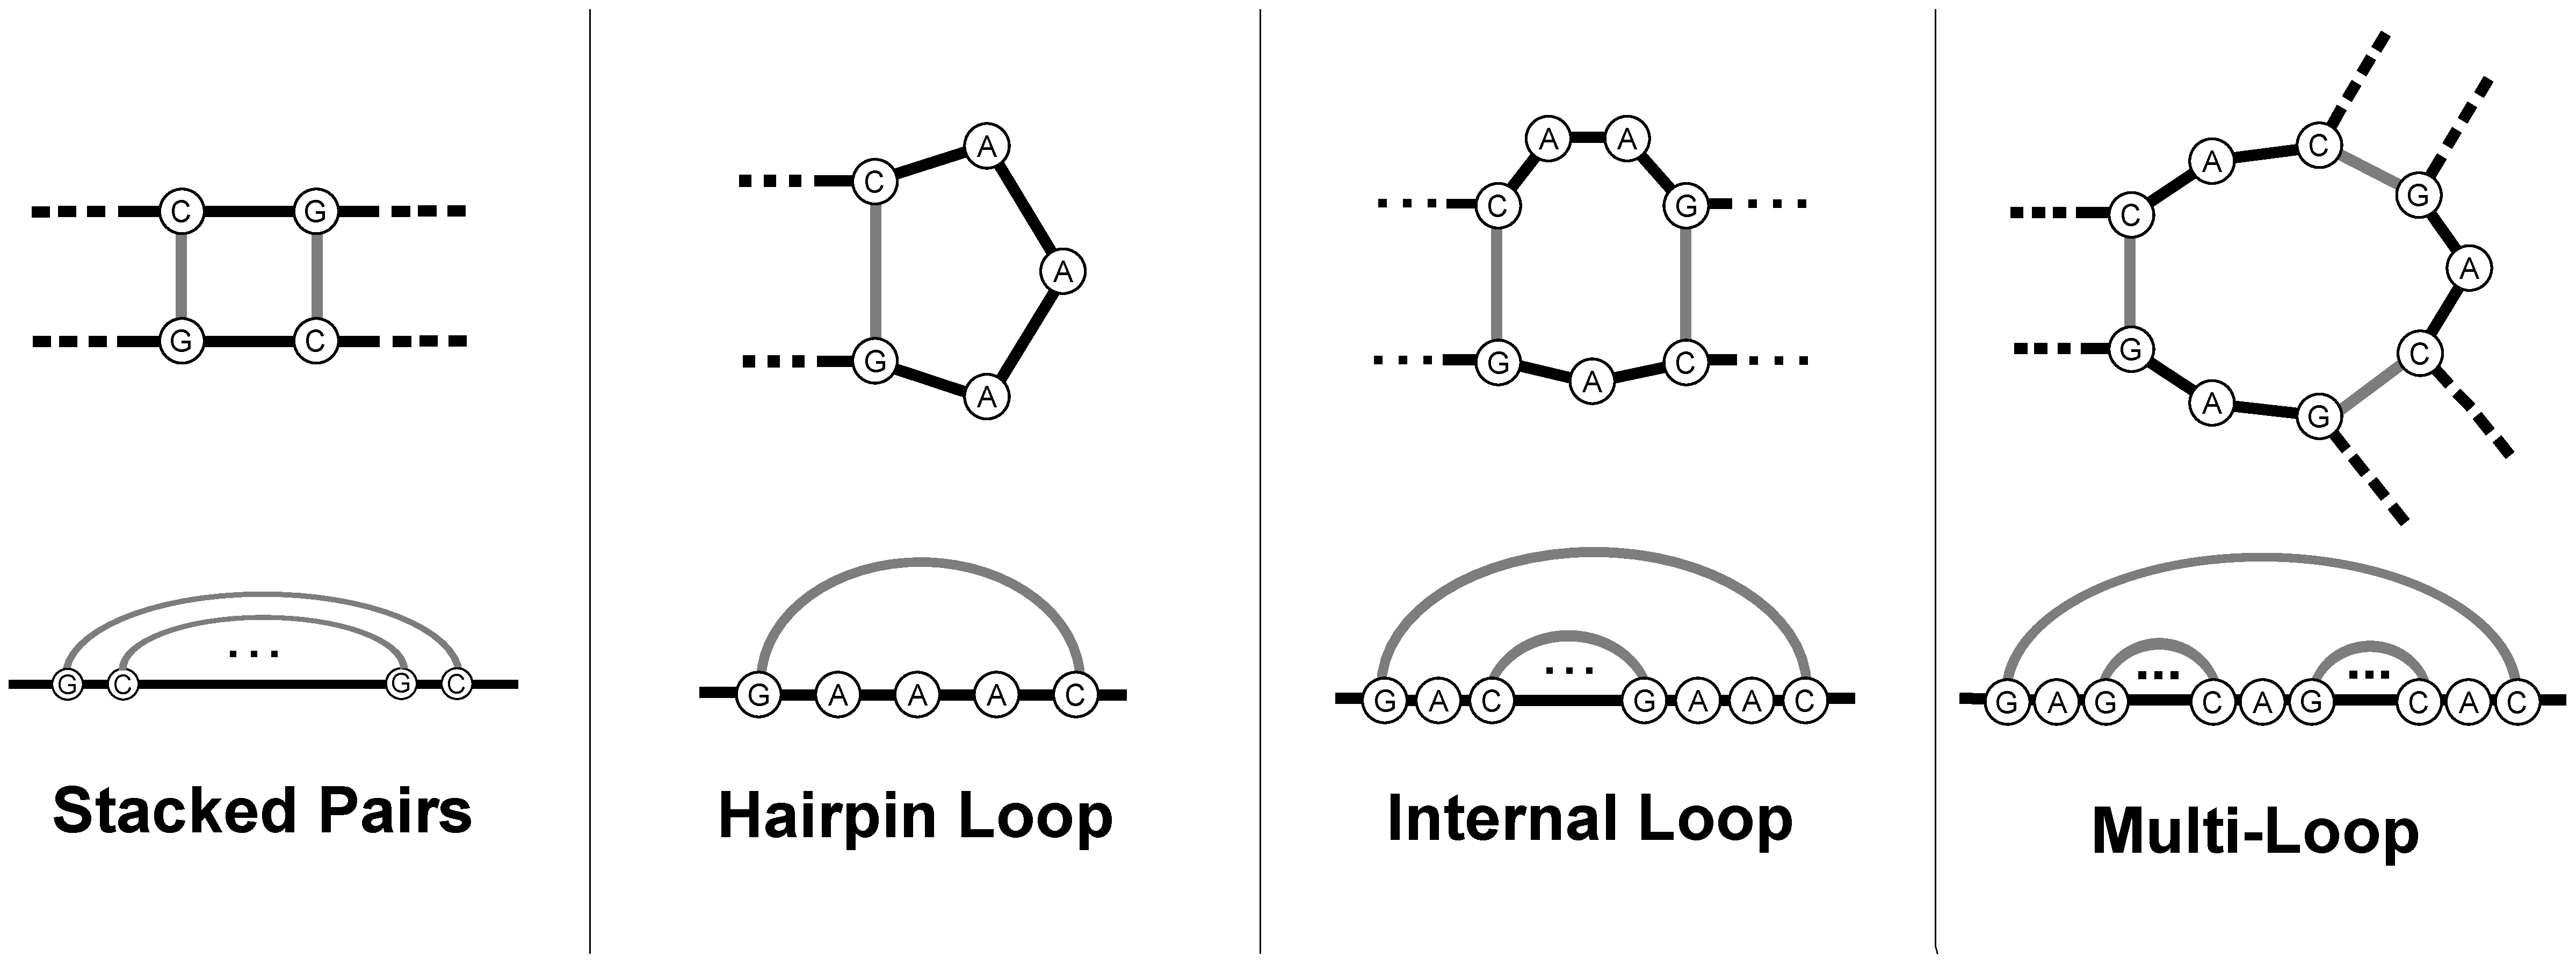
\includegraphics[width=\textwidth]{full_loop_figure.eps}
\caption{The 4 types of loops, black connections are bonds in the RNA
  backbone, grey connections are hydrogen bonds between bases. The
  types are: \textit{Stacked Pairs}, adjacent pairs of bonded bases,
  \textit{Hairpin Loops}, one bonding pair closing off a turn in the
  RNA backbone, \textit{Internal Loops}, which can range from bulges
  to long loops, connecting to pairs with 2 chains of unpaired bases,
  and \textit{Multi-Loops}, which  connect 3 or more pairs.}
\label{fig:loopFigure}
\end{figure}

\subsection{UV Melting Experiments} 

The individual loop regions are given energies as parameters to linear
regression models of free energy change in predictably folding
strands. For example, the strand `GGGAAACCC' folds predictably into a
structure with all the G's paired to the C's and a 3-A hairpin turn
(because G's pair very strongly to C's and A's tend to resist
pairing). Large amounts of identical strands are synthesized and put
into solution and heated. As the solution heats, there is enough
ambient energy to put all the strands in the unfolded, no-bonds
state. RNA is an organic, aromatic molecule that absobes light in the
UV spectrum in different amounts depending on whether it is in a
folded state or unfolded state, so the UV absobtion is fit to a curve
that then tells us about the relative concentrations of the
single-stranded vs. double-stranded state, which in turn tells us
about the free energy change between the two at a given
temperature. This free energy change is extracted and treated as a
function of the loop variables, which are then fitted to a linear
model over experiments on many different such strands.

To continue with the example, we are creating a model:

[TODO: example energy figure ]

\begin{equation}
\Delta G (GGGAAACCC) = \Delta G_s \left ( \begin{array}{c} 3' C C 5 ' \\ 5' G G 3 ' \end{array} \right ) +
\Delta G_S \left ( \begin{array}{c} 3' C C 5 ' \\ 5' G G 3 ' \end{array} \right ) +
\Delta G_H (G AAA C)
\end{equation}

Where $\Delta G_S $ is an individual parameter for the stack loop
energy term and $\Delta G_H$ contains the terms for the hairpin energy
term.

Briefly, the loop types are:
\begin{description}
\item[Stacked Pairs] Two pairs right next to each other. The energies
  for each possible legal pairing has been determined by linear
  regression on experimental data (see UV Melting
  Experiments). Finding an energy amounts to a table look-up of these
  regression coefficients.
\begin{equation}
  \Delta G \left ( \begin{array}{c} 5' G C 3'  \\ 3' C G 5' \end{array} \right ) = -3.42\text{ (from Xia et al 1998) } 
\end{equation}
\item[Hairpin Loops] One pair enclosing an empty loop region. The
  energy of this loop contains a term dependent on the length $n$, the
  sequence of the closing stack, and several bonus terms for special
  loops experimentally determined to be stable or unstable.
  \begin{equation}
    \begin{split}
      \Delta G_{Hairpin} (n > 3) =& \Delta G_{init}(n) + \Delta G(\text{closing stack})\\
      &+ \Delta G_{bonus} (\text{UU or GA first mismatch, but not AG} ) \\
      &+ \Delta G_{bonus} (\text{special GU closure} ) \\
      &+ \Delta G_{penalty} (\text{oligo-C loops}) \\
      & \text{(from Mathews et al 1999) }
    \end{split}
  \end{equation}
  For example (with $\bar{A}$ meaning base $A$ is unpaired):
  \begin{equation}
    \Delta G \left ( \begin{array}{c} 5' G \bar{A} \bar{A} 3' \\ 3' C \bar{A} \bar{A} 5' \end{array} \right )
    = \Delta
  \end{equation}


\item[Internal Loops] Two pairs connected by a loop.
  [TODO: add example]
\item[Multi Loops] Mutiple pairs, each with their own stems. This has
  a linear energy model, with an energy penalty for starting the loop,
  an energy term for each base pair, and one for each unpaired base.

\end{description}

\section{UV Melting Experiments}

The thermodynamic behavior of an RNA strand can be determined by
subjecting it to melting curve analysis. When a folded RNA strand
denatures, or unfolds because it is heated, its absorbtion of UV
radiation changes. A physical model of this melting process can be
developed to interpret these curves.

\begin{equation}
\Delta G = \Delta H + T \Delta S
\end{equation}

\begin{equation}
T_M^{-1} = \frac{R}{\Delta H} \log{(C_T/a)} + \frac{\Delta S}{R}
\end{equation}

The free energy of a loop structure, or rather its $\Delta G$ relative
to the unfolded state,

\paragraph{Stacked Pairs}

The energy parameters for stacked pair loops were computed in a series
of optical melting experiments (estimating parameters by UV
absorbtion) by Xia et al (1998). For each combination of 2 sets of 2
paired bases, the change in energy at 37 Kelven was computed by
fitting $\Delta H$ and $\Delta S$ to the data. [Todo: decide whether
to have an in depth discussion of this]

For GU, a non-cannonical base pair that happens nontheless, the free
energy is calculated by subtracting the free energy of a CGUACG strand
from the free energy of a CGUUGACG strand, both of whose free energies
are determined by optical melting experiments.


\paragraph{Dangling ends and terminal mismatches}

[TODO: read serra \& turner 1995]

bases adjacent to GU pairs are treated the same as bases adjacent to AU pairs

\paragraph{Hairpin loops}

The energy function for a hairpin loop is a similar table lookup.

[TODO: finish this]

- Tetraloop bonus

\paragraph{Bulge loops}

\paragraph{Internal loops}
- 2x2 tandem mismatches
- 2x1 internal loops
- 1x1 (single mismatch

